\documentclass[main.tex]{subfiles} 
\begin{document}

% see this for  guidance https://www.cs.purdue.edu/homes/dec/essay.dissertation.html
\section{EXAMPLES}
    
    The following are examples of some elements that might be included in a dissertation.

    \subsection{TABLES}
        
        The tables will also span nicely across pages when necessary. 
    
        \begin{longtable}{@{}l rr rr}
            % pairs: absolute number (percentage)
            
            \toprule%
             \centering%
             {\bfseries Student}
             & {\bfseries Course}
             & {\bfseries Score} \\
            
            \cmidrule[0.4pt](r{0.125em}){1-1}%
            \cmidrule[0.4pt](lr{0.125em}){2-2}%
            \cmidrule[0.4pt](l{0.125em}){3-3}%
            % \midrule
            \endhead
            
            Pam VanDeMark & Mathematics & 87 \\
            \myrowcolour%
            Max Anderson & Reading & 91 \\
            Julia & Biology & 68 \\
            \myrowcolour%
            Teddy & Physics & 89 \\ 
            Pat Thompson & Literature & 87 \\ 
            \myrowcolour%
            Max & Gym  & 45 \\ 
            Sari & Art  & 100 \\
            
            \bottomrule
            
            \caption{STUDENT COURSE GRADES}
            \label{tab:grades}
        \end{longtable}
        
        Below is an example of a table with longer text in each box.
    
        \begin{longtable}{p{3cm}p{11cm}}
                \toprule%
                 \centering%
                 {\bfseries Some Topic}
                 & {\bfseries Description of Topic} \\
                
                \cmidrule[0.4pt](r{0.125em}){1-1}%
                \cmidrule[0.4pt](lr{0.125em}){2-2}%
                % \midrule
                \endhead
                
                Very Long Title Topic & Per ne posse nonumy persius, etiam movet epicuri 
                vix ne. Ea his omnesque rationibus omittantur. In eam lucilius adolescens, 
                ad tincidunt voluptatibus mediocritatem pro. Mel ad hinc libris, quo 
                soleat moderatius at. Mea accusata incorrupte ex, ne vim putant mediocrem. \\
                \myrowcolour%
                Another Topic & No quo tacimates interesset. Eruditi voluptua ut nam, 
                his ut mutat saepe. Et has purto ferri everti, eum facer semper insolens 
                an. Quo prima veniam aperiam in, sumo fastidii intellegebat pri ex, 
                augue feugiat accommodare qui te. \\
                Final Topic & Vivendum menandri sit te, quo id option voluptatibus. 
                Et his nisl elitr persecuti. Vix nihil complectitur te, est error 
                altera molestie ex. Novum deleniti nam ea.  \\
                
                \bottomrule
                
                \caption{SOME TOPICS}
                \label{tab:topics}
            \end{longtable}
            
    \subsection{IMAGES}
        Images are fairly easy to include in a \LaTeX document.  
        Figure \ref{fig:facvsphd} provides an example.  The figure comes from
        an article in 2013 \cite{Schillebeeckx2013}.
        
        \begin{figure}[ht]
            \centering
            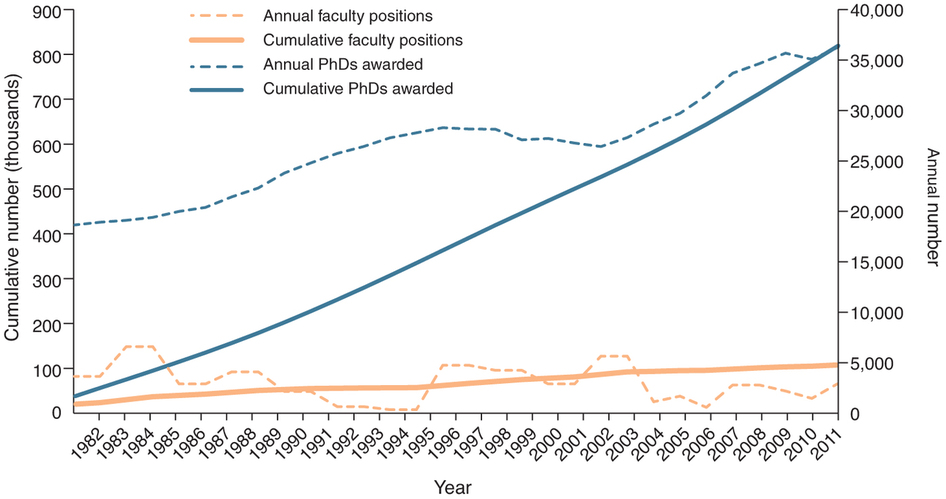
\includegraphics[scale=.4]{images/facultyVsPhd.jpg}
            \caption{NEW FACULTY POSITIONS VERSUS NEW PHDS}
            \label{fig:facvsphd}
        \end{figure}
    
    \subsection{LISTS}
        
        Various lists can be included in a dissertation.  Here are some examples. 
        
        \subsubsection{PLAIN LIST}
            Below is very simple example of a basic list.
            \begin{itemize}
                \item Some Item
                \item Different Item
                \item More Different Item
                \item Another Great Item
            \end{itemize}
            
        \subsubsection{NUMBERED LIST}
        
            \begin{enumerate}
                \item Automatically
                \item Numbered 
                \item For 
                \item You
            \end{enumerate}
            
        \subsubsection{NESTED LIST}
            Below is a different example of creating a nested list. 
            If you create a lot of nested lists, using \textit{easylist}
            can definitely save you time.

            \begin{easylist}[itemize]
                & Item
                && SubItem
                && SubItem
                & Item
                && SubItem
                && SubItem 
                && SubItem
                & Another Item
                && SubItem
                && SubItem
                & Final Item
            \end{easylist}
            
        \subsubsection{DEFINITION LIST}
            The following is a list of definitions.  Not all dissertations will contain
            such a list, but it is acceptable.  Below is an acceptable format for
            listing a few definitions. 
            
            \begin{description}
                \item[Dissertation] - a written essay, treatise, or thesis, 
                    especially one written by a candidate for the degree of 
                    Doctor of Philosophy (PhD) \nomenclature{PhD}{Doctor of Philosophy}
                \item[Mathematics] - the systematic treatment of magnitude, relationships 
                    between figures and forms, and relations between quantities 
                    expressed symbolically. 
                \item[Statistics] - the science that deals with the collection, 
                    classification, analysis, and interpretation of numerical 
                    facts or data, and that, by use of mathematical theories of 
                    probability, imposes order and regularity on aggregates of 
                    more or less disparate elements
            \end{description}
    
    \subsection{ABBREVIATIONS}
        This template includes the \textit{nomencl} package which makes creating a 
        list of abbreviations very easy.  Suppose you wanted
        to abbreviate South Dakota State University 
        (SDSU) \nomenclature{SDSU}{South Dakota State University}. Just add 
        \begin{verbatim}
            \nomenclature{SDSU}{South Dakota State University}
        \end{verbatim}
        after your first use of the abbreviation.  Then an abbreviation page 
        will automatically be created with the abbreviations.  It page will 
        also be alphabetical regardless of the order of abbreviations in the 
        document.
    
    \subsection{REFERENCE OTHER LOCATIONS IN DOCUMENT}
    
        \LaTeX provides a very simple strategy for referencing others parts
        in the document.  For example, you can easily reference Appendix \ref{app:extra}.  
        Just include 
        \begin{verbatim}
            \label{YourLabelName}
        \end{verbatim}
        where you want to reference. Then just use the following to reference that
        location.
        \begin{verbatim}
            \ref{YourLabelName}
        \end{verbatim}
        
    \subsection{MATH FORMULAS}
        Honestly, if you are using \LaTeX, math formulas should be nothing
        new.  In any case, here is a simple example.
        
        \begin{displaymath}
           V = \left\{
             \begin{array}{lr}
               \text{where } A_i ==  B_i  & :  10 \cdot k \\
               \text{where } A_i \leq B_i & : \frac{B_i - A_i}{B_i}\cdot k \\
               \text{where } A_i > B_i  & : \frac{(A_i - B_i)^2 }{k \cdot \sqrt{\pi}}
             \end{array}
           \right. \text{   , some fancy formula}
        \end{displaymath}
        

\end{document}